\documentclass[letter,12pt]{article}
\usepackage[paperheight=27.94cm,paperwidth=21.59cm,bindingoffset=0in,left=3cm,right=2.0cm, top=3.5cm,bottom=2.5cm, headheight=200pt, headsep=1.0\baselineskip]{geometry}
\usepackage{graphicx,lastpage}
\usepackage{upgreek}
\usepackage{censor}
\usepackage[spanish,es-tabla]{babel}
\usepackage{pdfpages}
\usepackage{tabularx}
\usepackage{graphicx}
\usepackage{adjustbox}
\usepackage{xcolor}
\usepackage{colortbl}
\usepackage{rotating}
\usepackage{multirow}
\usepackage[utf8]{inputenc}
\usepackage{float}
\usepackage{verbatim}
\usepackage{listings}

\lstset{
  basicstyle=\ttfamily\footnotesize,
  breaklines=true,
  frame=single,
  columns=fullflexible
}

\renewcommand{\tablename}{Tabla}
\usepackage{fancyhdr}
\pagestyle{fancy}


%
\begin{document}
%
   \title{\Huge{Informe Laboratorio 1}}

   \author{\textbf{Sección 4} \\  \\Luciano Silva Rivas \\ e-mail: luciano.silva@mail.udp.cl}
          
   \date{Septiembre de 2026}

   \maketitle
   
   \tableofcontents
 
  \newpage
  

\section{Descripción}

\begin{enumerate}
    \item  Usted empieza a trabajar en una empresa tecnológica que se jacta de poseer sistemas que permiten identificar filtraciones de información a través de Deep Packet Inspection (DPI).
    A usted le han encomendado auditar si efectivamente estos sistemas son capaces de detectar las filtraciones a través de tráfico de red. Debido a que el programa ping es ampliamente utilizado desde dentro y hacia fuera de la empresa, su tarea será crear un software que permita replicar tráfico generado por el programa ping con su configuración por defecto, pero con fragmentos de información confidencial. Recuerde que al comparar tráfico real con el generado no debe gatillar alarmas.
    De todas formas, deberá hacer una prueba de concepto, en la cual se demuestre que al conocer el algoritmo, será fácil determinar el mensaje en claro.
    Para los pasos 1,2,3 indicar el texto entregado a ChatGPT y validar si el código resultante cumple con lo requerido.


\end{enumerate}


\section{Actividades}


\subsection{Algoritmo de cifrado}

\begin{enumerate}
\item Generar un programa, en python3 utilizando chatGPT, que permita cifrar texto utilizando el algoritmo Cesar. Como parámetros de su programa deberá ingresar el string a cifrar y luego el corrimiento.
\begin{figure}[H]
        \centering
        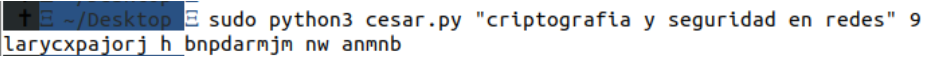
\includegraphics[width=15cm]{actividades/A1.png}
        \label{fig:a1}
\end{figure}


\end{enumerate}

\subsection{Modo stealth}

\begin{enumerate}
    \item Generar un programa, en python3 utilizando ChatGPT, que permita enviar los caracteres del string (el del paso 1) en varios paquetes ICMP request (un caracter por paquete en el campo data de ICMP) para de esta forma no gatillar sospechas sobre la filtración de datos.
Deberá mostrar los campos de un ping real previo y posterior al suyo y demostrar que su tráfico consideró todos los aspectos para pasar desapercibido.
    \begin{figure}[H]
        \centering
        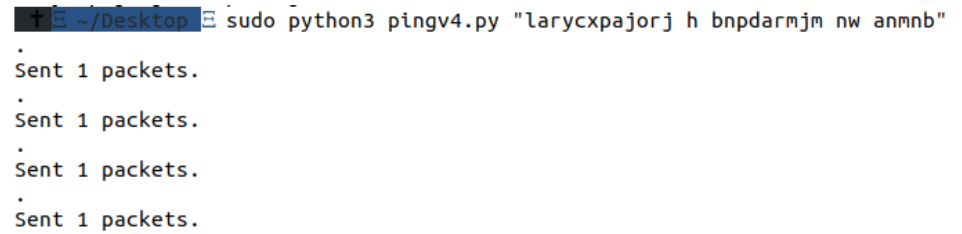
\includegraphics[width=15cm]{actividades/A2.1.png}
        \label{fig:a2-1}
    \end{figure}
    El último carácter del mensaje se transmite como una b.
    \begin{figure}[H]
            \centering
            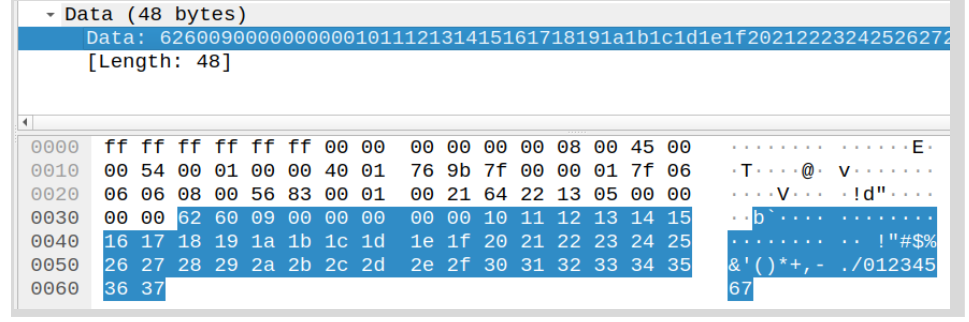
\includegraphics[width=15cm]{actividades/A2.2.png}
            \label{fig:a2-2}
        \end{figure}
\end{enumerate}

\subsection{MitM}
\begin{enumerate}
    \item Generar un programa, en python3 utilizando ChatGPT, que permita obtener el mensaje transmitido en el paso2. Como no se sabe cual es el corrimiento utilizado, genere todas las combinaciones posibles e imprímalas, indicando en verde la opción más probable de ser el mensaje en claro.
    \begin{figure}[H]
        \centering
        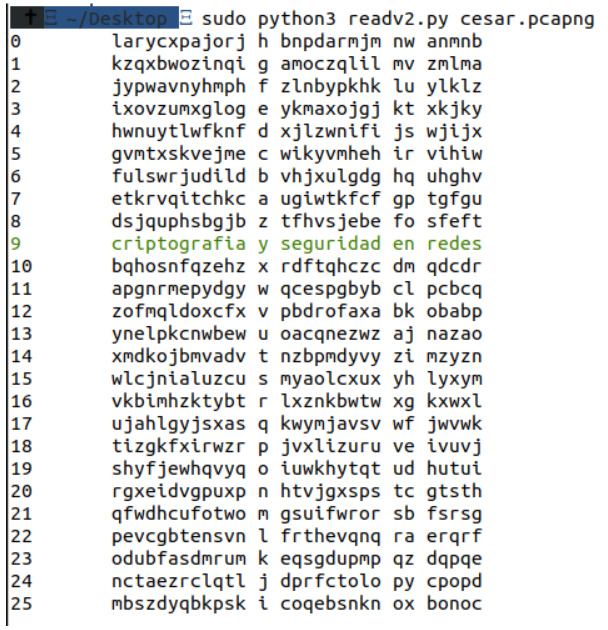
\includegraphics[width=12cm]{actividades/A3.png}
        \label{fig:a3}
    \end{figure}
    Finalmente, deberá indicar 4 issues que haya tenido al lidiar con ChatGPT, netamente para reflejar cuál fue su experiencia al trabajar con esta tecnología.

\end{enumerate}

\section{Desarrollo de Actividades}

\subsection{Actividad 1}

\textbf{Prompt entregado a la IA:} ``Genera un programa en Python3 llamado \texttt{cesar.py} que reciba dos argumentos desde la terminal: un texto a cifrar y un corrimiento (número entero). El programa debe cifrar el texto usando el algoritmo de César, dejando espacios, números y símbolos sin modificar, y respetando mayúsculas y minúsculas. Debe imprimir el resultado por pantalla.''

\textbf{Código obtenido:}
\lstinputlisting[language=Python, caption={cesar.py}]{scripts/cesar.py}

\textbf{Validación:} al ejecutar \verb|python3 cesar.py "criptografia y seguridad en redes" 9| se obtuvo \texttt{larycxpajorj h bnpdarmjm nw anmnb} (Figura \ref{fig:a1-resultado}), que coincide exactamente con el resultado esperado en el enunciado. El código recibe los argumentos por terminal y logra el cifrado César correctamente, cumpliendo ambos criterios de esta actividad sin necesidad de corrección.

\begin{figure}[H]
    \centering
    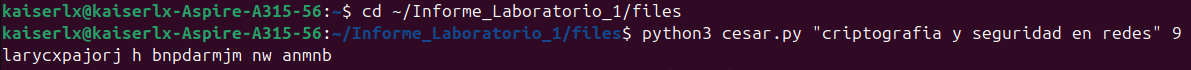
\includegraphics[width=12cm]{actividades/A1_resultado.png}
    \caption{Ejecución de cesar.py}
    \label{fig:a1-resultado}
\end{figure}

\subsection{Actividad 2}

\textbf{Prompt entregado a la IA:} ``Genera un programa en Python3 llamado \texttt{pingv4.py} que use scapy para enviar un string carácter por carácter, un carácter por paquete ICMP echo request, hacia una IP de loopback, uno por segundo. El payload de cada paquete debe medir 48 bytes -igual que un ping real en este equipo- y no solo el carácter: el carácter va en el primer byte, seguido de 2 bytes de relleno variables, 5 bytes en 0x00, y el patrón fijo 0x10 a 0x37 que usa ping por defecto, para no diferenciarse en tamaño de un ping real. El id ICMP debe mantenerse fijo durante toda la ejecución y el id IP debe ser incremental, igual que en un ping real.''

\textbf{Código obtenido:}
\lstinputlisting[language=Python, caption={pingv4.py}]{scripts/pingv4.py}

\textbf{Validación:} el código generado inicialmente no cumplía todos los requisitos y debió corregirse dos veces (ver Issues 1 y 3 en las conclusiones). La versión final sí cumple con la rúbrica del laboratorio:
\begin{itemize}
    \item Envía el tráfico a la IP de loopback (\texttt{127.0.0.1}), pasada como argumento.
    \item Inyecta el carácter cifrado en el primer byte del payload ICMP.
    \item Mantiene la ejecución a un envío por segundo (\texttt{time.sleep(1.0)}).
    \item El id IP es incremental y el id ICMP se mantiene fijo durante toda la sesión, igual que hace un ping real.
    \item El número de secuencia ICMP es incremental (1, 2, 3\ldots).
    \item El payload respeta la estructura de 3 bytes coherentes + 5 bytes en 0x00 + patrón 0x10 a 0x37 (48 bytes en total).
    \item El checksum es calculado automáticamente por scapy al construir el paquete (\texttt{Checksum Status: Good} en la Figura \ref{fig:a2-payload}).
\end{itemize}

Un hallazgo adicional de la auditoría: los paquetes del canal encubierto miden 90 bytes en total (Figura \ref{fig:a2-payload}), mientras que un ping real en este equipo mide 98 bytes -8 bytes de diferencia, porque el payload por defecto de \texttt{ping} en este sistema es de 56 bytes y el nuestro, siguiendo la estructura pedida, es de 48. La estructura interna del payload coincide con la esperada, pero no logra igualar el largo exacto de un ping real, lo que en un sistema DPI real seguiría siendo una señal detectable.

\begin{figure}[H]
    \centering
    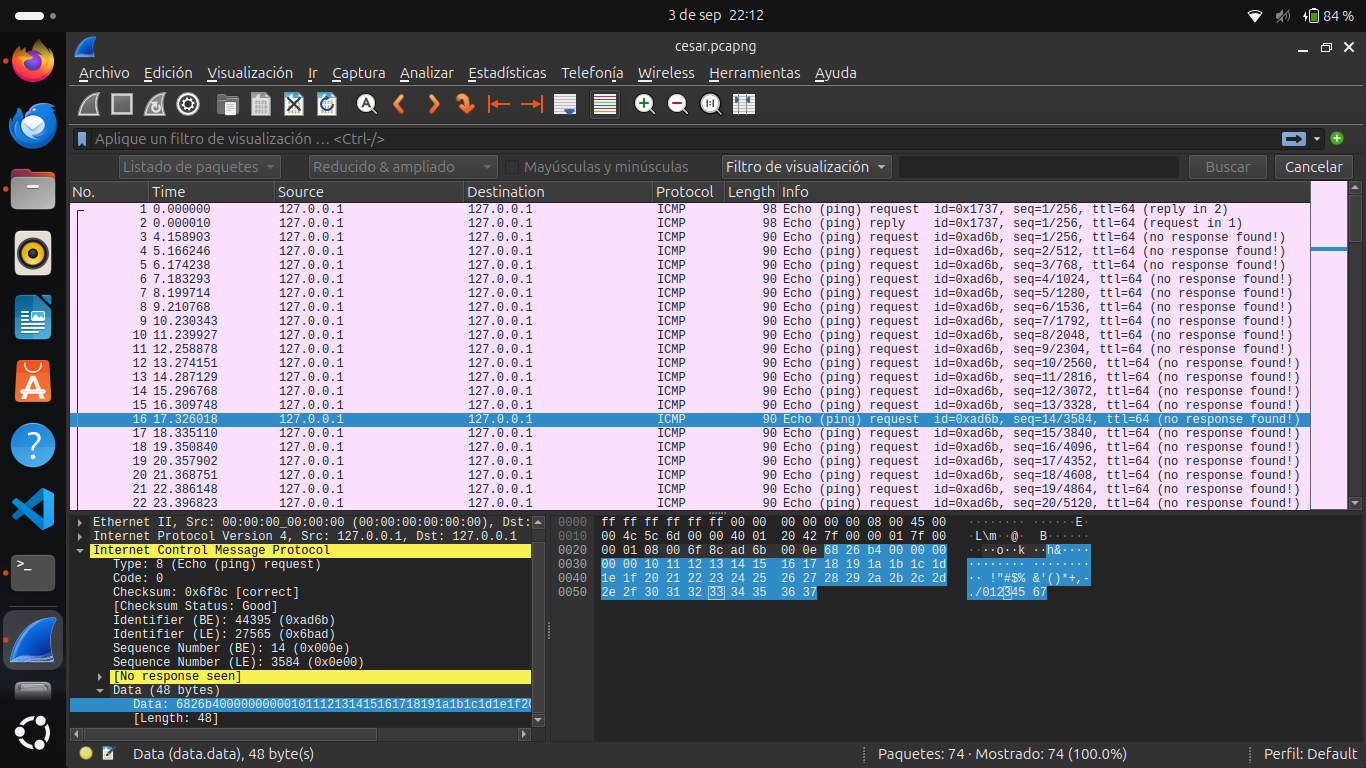
\includegraphics[width=15cm]{actividades/A2_wireshark_payload.png}
    \caption{Captura en Wireshark: tráfico completo y detalle del payload de un paquete del canal encubierto (paquete \#16, carácter \texttt{'h'}, byte 0 = 0x68)}
    \label{fig:a2-payload}
\end{figure}

\subsection{Actividad 3}

\textbf{Prompt entregado a la IA:} ``Genera un programa en Python3 llamado \texttt{readv2.py} que reciba como argumento un archivo pcap, reconstruya el string enviado por \texttt{pingv4.py} identificando sus paquetes por la estructura del payload (48 bytes, terminados en el patrón 0x10 a 0x37, con 5 bytes en 0x00), y luego pruebe las 26 combinaciones posibles de descifrado César sobre ese string, imprimiéndolas todas y destacando en verde tanto el texto en claro como el corrimiento (llave) más probable, usando análisis de frecuencia de letras en español.''

\textbf{Código obtenido:}
\lstinputlisting[language=Python, caption={readv2.py}]{scripts/readv2.py}

\textbf{Validación:} ejecutando \texttt{sudo python3 readv2.py cesar.pcapng} sobre la captura completa (que incluye también los pings reales de antes/después) se recuperan las 26 combinaciones y se destaca en verde el corrimiento 9 junto al mensaje en claro \texttt{criptografia y seguridad en redes}, que corresponde exactamente al texto original de la Actividad 1 (Figura \ref{fig:a3-resultado}). El filtro por estructura del payload evita que los pings reales mezclados en el mismo pcap contaminen el mensaje reconstruido; además fue necesario descartar duplicados por número de secuencia (ver Issue 2 en las conclusiones), ya que la interfaz \texttt{lo} captura cada paquete dos veces.

\begin{figure}[H]
    \centering
    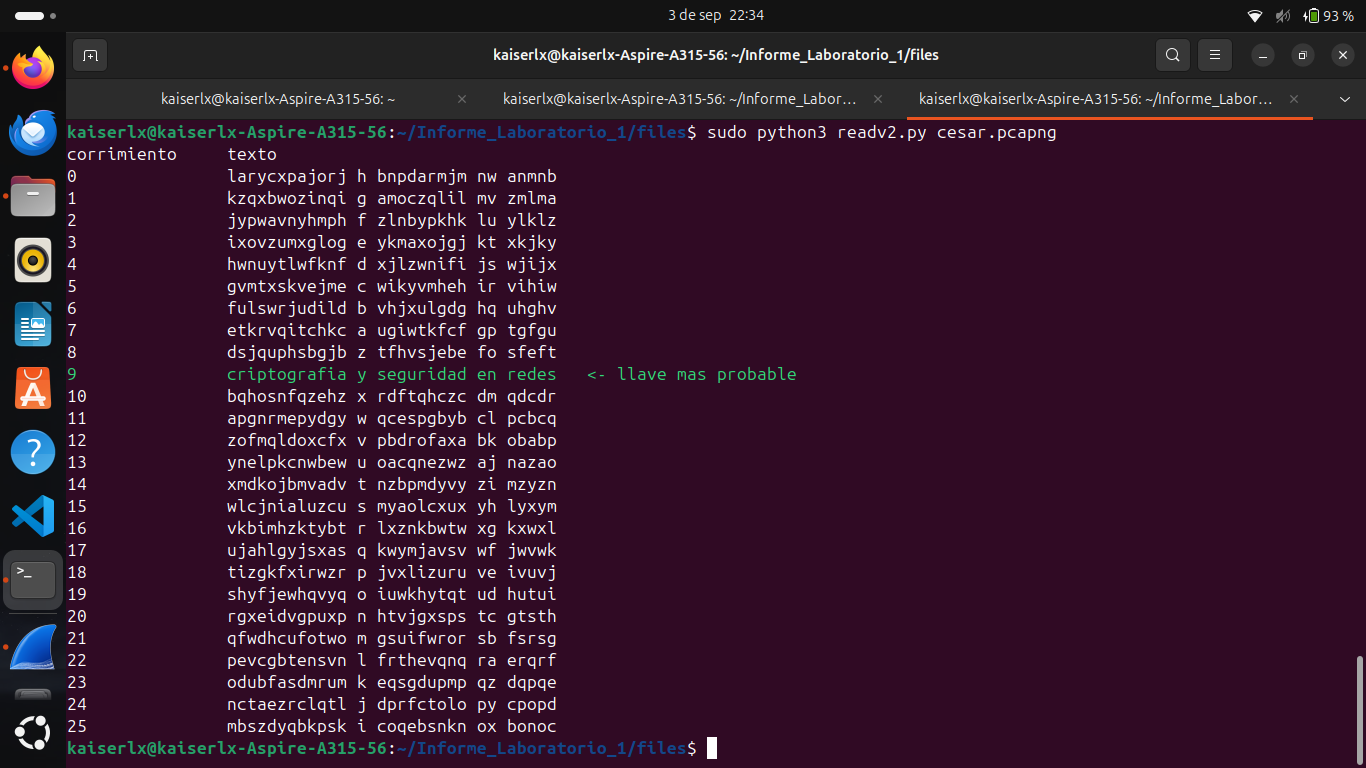
\includegraphics[width=12cm]{actividades/A3_resultado.png}
    \caption{Salida de readv2.py: las 26 combinaciones, con el corrimiento correcto en verde}
    \label{fig:a3-resultado}
\end{figure}


% Please add the following required packages to your document preamble:
%\begin{table}[htbp]

\section*{Conclusiones y comentarios}

A partir del desarrollo de la actividad fue posible implementar de extremo a extremo un canal de exfiltración de datos utilizando tráfico ICMP, junto con una herramienta capaz de recuperar el mensaje original a partir de la captura de tráfico. El trabajo permitió comprobar que, si bien la implementación básica del canal resulta relativamente sencilla, conseguir que los paquetes generados presenten características similares a las de un tráfico ICMP legítimo requiere considerar varios aspectos adicionales.

Durante el desarrollo se identificaron principalmente cuatro problemas:

\begin{enumerate}
\item \textbf{Espera innecesaria de respuestas durante el envío.} La primera versión de \texttt{pingv4.py} utilizaba \texttt{sr1()} para enviar cada paquete y esperar una respuesta durante un máximo de 2 segundos. Debido a que los paquetes generados no necesariamente recibían una respuesta, el tiempo total de ejecución superaba los 80 segundos, dando la impresión de que el programa se encontraba detenido. Para solucionar este problema se reemplazó \texttt{sr1()} por \texttt{send()}, dado que para los objetivos de la actividad solo era necesario realizar el envío de los paquetes y no esperar una respuesta individual por cada uno.

```
\item \textbf{Problemas en la reconstrucción del mensaje.} Al utilizar la captura completa \texttt{cesar.pcapng}, el programa también procesaba los pings reales realizados antes y después del envío del mensaje. Como estos paquetes podían utilizar un número de secuencia igual a 1, eran interpretados como parte del canal encubierto, generando caracteres adicionales en el mensaje reconstruido. Una vez corregido este problema, se identificó una segunda dificultad relacionada con la interfaz de loopback. En la captura, cada paquete podía aparecer tanto como tráfico de salida como de entrada, provocando que cada carácter fuera procesado dos veces y que el mensaje apareciera duplicado, por ejemplo, como \texttt{ccrriippttooggrraaffiiaa...}. Para solucionarlo se incorporó un filtro basado en la estructura del payload, permitiendo diferenciar los paquetes del canal respecto del tráfico ICMP normal. Además, se descartaron números de secuencia repetidos para evitar procesar dos veces el mismo carácter.

\item \textbf{Diferencia en el tamaño del payload.} En la primera implementación se utilizaba únicamente el carácter cifrado como contenido del payload, por lo que este tenía un tamaño de 1 byte. Esto generaba una diferencia considerable respecto de los pings normales observados en el equipo, cuyos paquetes tenían un tamaño de payload de 48 bytes. Esta diferencia podía utilizarse fácilmente como característica para distinguir el tráfico generado. Para reducir esta discrepancia se modificó la estructura del payload, manteniendo un tamaño constante de 48 bytes y almacenando el carácter cifrado dentro de los primeros bytes.

\item \textbf{Inconsistencias en los campos de IP e ICMP.} Otro de los problemas encontrados estuvo relacionado con los valores utilizados en los encabezados de los paquetes. Las primeras versiones no reproducían de manera suficientemente consistente el comportamiento observado en un ping real, particularmente en aspectos como el identificador ICMP, el identificador IP y los números de secuencia. Por esta razón, fue necesario modificar la generación de los paquetes para que estos campos siguieran un comportamiento coherente con el tráfico legítimo. Las modificaciones fueron posteriormente contrastadas con capturas obtenidas mediante Wireshark y con los criterios establecidos en la rúbrica de la actividad.
```

\end{enumerate}

En términos generales, la utilización de IA fue útil durante las primeras etapas del desarrollo, principalmente para obtener rápidamente una versión inicial y funcional de los distintos scripts. Sin embargo, las soluciones generadas inicialmente no cumplían todos los requisitos de la actividad, por lo que fue necesario realizar un proceso de prueba y corrección. Esto implicó ejecutar los programas, analizar las capturas obtenidas mediante Wireshark, compararlas con tráfico ICMP real y modificar los scripts según los problemas encontrados.

Finalmente, uno de los principales aprendizajes de la actividad fue que la implementación del canal de comunicación no constituye necesariamente la mayor dificultad. El desafío más importante estuvo en reducir las diferencias entre el tráfico generado y el comportamiento de un ping legítimo. Aspectos como el tamaño de los paquetes, la estructura del payload y la coherencia de los campos de los encabezados pueden ser suficientes para distinguir un tráfico anómalo. Por lo tanto, el ejercicio permitió comprender de manera práctica la importancia de analizar no solo la funcionalidad de un canal encubierto, sino también las características que pueden hacerlo detectable.


\end{document}
